\PassOptionsToPackage{quiet}{xeCJK}
\documentclass[declarePage]{ecnuthesis}
% 模版选项
% 模版选项是指在导入文档类的时候所指定的选项
% \documentclass[<模版选项>]{ecnuthesis}
% 可用的模版选项:
%   printMode     是否开启打印模式, 若缺省则为关闭, 反之则为开启
%   declarePage   是否生成声明页, 若缺省则不生成, 反之则生成
% 用法示例
%   \documentclass[printMode]{ecnuthesis}   (开启打印模式, 适合双面打印)
%   \documentclass{ecnuthesis}              (关闭打印模式, 适合提交电子版)

\ecnuSetup {
% 参数设置
% 允许采用两种方式设置选项:
%   1. style/... = ...
%   2. style = { ... = ... } 
% 注意事项: 
%   1. 请勿在参数设置中出现空行
%   2. "=" 两侧的空格将被忽略
%   3. "/" 两侧的空格不会被忽略
%   4. 请使用英文逗号 "," 分隔选项
%
% info 类用于输入论文信息
info = {
    title = {晶格动力学学习报告},
    % 中文标题
    %
    titleEN = {Lattice Dynamics Learning Report},
    % 英文标题
    %
    author = {刘光远},
    % 作者姓名
    %
    studentID = {10222150413},
    % 作者学号
    %
    department = {通信与电子工程学院},
    % 学院名称
    %
    major = {微电子科学与工程},
    % 专业名称
    %
    supervisor = {翁国恩},
    % 指导教师姓名
    %
    academicTitle = {副教授},
    % 指导教师职称
    %
    year  = 2022,
    % 论文完成年份
    %
    month = 11,
    % 论文完成月份
    %
    graduationYear = 22,
    % 内封面毕业届别
    % 说明:
    %   若 graduationYear 字段为空,则内封面毕业届别为 year
    %
    keywords = {晶格动力学,晶格振动,声子,声子热容,},
    % 中文关键词
    % 请使用英文逗号 "," 以分隔
    %
    keywordsEN = {x},
    % 英文关键词
    % 请使用英文逗号 "," 以分隔
    %
},
% style 类用于简单设置论文格式
style = {
    footnote  = plain,
    % 脚注编号样式
    % 可用选项:
    %   footnote = plain|circled
    % 说明:
    %   plain     脚注的编号仅为数字
    %   circled   脚注的编号为带圆圈数字 (仅限1-10)
    %   (默认选项为 plain )
    %
    numbering = arabic,
    % 章节编号样式
    % 可用选项:
    %   numbering = arabic|alpha|chinese
    % 说明:
    %   arabic    使用数字进行编号 (即理科要求)
    %   alpha     使用字母进行编号 (即外文要求)
    %   chinese   使用汉字进行编号 (即文科要求)
    %   (默认选项为 arabic )
    %
    fontCJK = fandol,
    % 中文字体选择
    % 可用选项:
    %   fontCJK = fandol|windows|mac
    % 说明:
    %   fandol    使用 TeX 自带的 fandol 字体
    %   windows   使用 Windows 系统内的字体 (中易)
    %   mac       使用 MacOS 系统内的字体
    %   (默认选项为 fandol )
    %
    fontMath = times,
    % 数学字体选择
    % 可用选项:
    %   fontMath = lm|times
    % 说明:
    %   lm        使用 TeX 自带的 Latin Modern 数学字体
    %   times     使用 Times 风格的数学字体
    %   (默认选项为 lm )
    %
    % declarePageResource = {./source/declaration.pdf},
    % 扫描版声明页 PDF 文件
    % 若该值为空则生成模版预定义的声明页;否则将插入指定路径所对应的 PDF 文件
    % 默认值为空
    %
    bibResource = {./source/thesis-ref.bib},
    % 参考文献数据源
    % 由于使用的是 biber + biblatex , 所以必须明确给出 .bib 后缀名
    %
    logoResource = {./source/inner-cover(contains_font).eps},
    % 封面插图数据源
    % 模版已自带, 位于 ./source/inner-cover(contains_font).eps
    % 默认值为空
}
}

% 需要的宏包可以自行调用
\usepackage{mwe}
\usepackage{zhlipsum}
\usepackage{makecell}

%声明图片路径
\graphicspath{{figures/}}







\begin{document}

% 设置前置部分编号
\frontmatter

% 中文摘要环境
\begin{abstract}
本篇学习报告主要记录学习晶格动力学的过程和心得。晶格动力学是在波恩-奥本海默近似的基础上展开研究的
\end{abstract}

% 英文摘要环境


% 设置正文编号
\mainmatter

\chapter{问题导向} 

对于大部分固体而言,在室温附近或在比较高的温度下,它的摩尔热容都是一个固定值$3R$($R$是理想气体常数),具体值为24.6$J/mol \cdot K$。%
从能量均分学说的角度出发,在经典理论中这一规律由杜隆-珀蒂定律概括。\cite{xxx}

事实上,多数晶体在室温或高温下,热容的实验值十分吻合,如下图\ref{HC}所示。但随着温度下降,实验发现固体热容随温度同时下降。%
所以在较低的温度下,热容随温度下降而下降的现象,经典的杜隆-珀蒂定律无法解释。
\begin{figure}[htb]
    \centering
    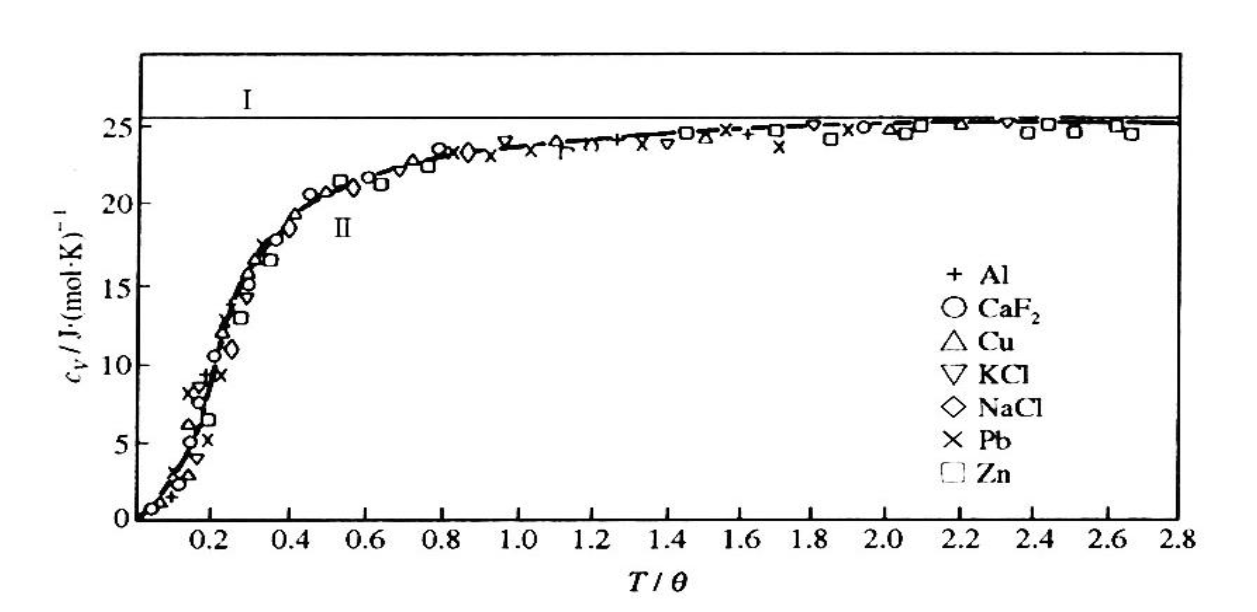
\includegraphics[width=.7\textwidth]{HC.png}
    \bicaption{固体热容实验值与理论值的比较}{Comparison Between Experiment and Theory of Heat Capacity}\label{HC}
\end{figure}

因此,围绕晶格动力学重新研究原子的运动,从而认识到原子运动对晶体的热性质(如热容)的影响,就是本次学习报告重点关注的方向。

\chapter{波恩-奥本海默近似 (Born-Oppenheimer Approximation)}

晶体表现出来的各种物理性质,背后的物理原理在于其中组成具体的基本粒子的运动规律,如原子和电子。%
以钠晶体为例,其中基本粒子的数量级在$10^{23}$,而基本粒子之间又存在着相互作用,要去考察他们各自的运动规律,%
从数学上来讲,这个多体问题是很难有严格解的。

因此,如图\ref{BOA}所示,采用波恩-奥本海默近似来简化分析,将电子运动和原子核运动分开处理。%
当我们考虑原子运动时,就不再关注电子是如何运动的;考虑电子运动的时候也同理。有关前者的研究就是本次报告的主题——晶格动力学。
\begin{figure}[htb]
    \centering
    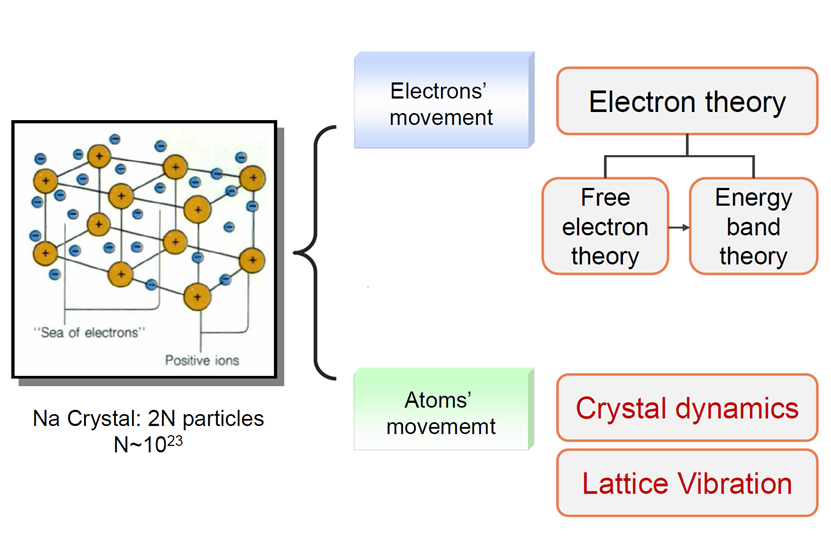
\includegraphics[width=.7\textwidth]{BOA.png}
    \bicaption{波恩-奥本海默近似}{Born-Oppenheimer Approximation}\label{BOA}
\end{figure}

\chapter{晶格振动 (Lattice Vibration)}

在晶体中,原子都是呈周期性排列,周期排列形成的点阵就是晶格,每个晶格的位置都是原子的平衡位置,所有的原子都在平衡位置做微小的振动。%
本章为研究晶格振动的基本原理,先从一维单原子链入手,分析其运动方程、边界条件、色散关系、格波形式等等,%
之后分析一维双原子相关问题并推广到三维。%
最后,对格波进行量子化分析,引入声子这个概念,从而能够方便地计算晶格振动能量。

\section{一维单原子链 (1D Monoatomic Chain)}

如图 \ref{1DMC} 所示,假设一个晶格常数为a,有$N$个原胞的一维单原子链,每个原胞内只有一个原子,为研究方便,先做以下两个假设:

简谐假设,原子做简谐振动,原子之间作用力为简谐力,该力满足
\begin{equation}
    F = - \beta x \text{;}
\end{equation}
最近邻假设,即原子只和最近邻原子有相互作用。
\begin{figure}[htb]
    \centering
    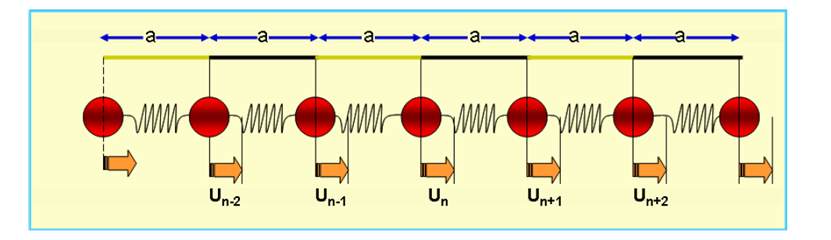
\includegraphics[width=.7\textwidth]{1DMC.png}
    \bicaption{一维单原子链}{1D Monoatomic Chain}\label{1DMC}
\end{figure}

在以上假设的基础上,对该模型进行如下分析。

\subsection{运动方程 (Equation of Motion)}

对一维单原子链中第n个原子进行受力分析,即可得到它的运动方程。根据牛顿第二定律和胡克定律,有
\begin{equation}
    m \ddot{u}_n = \beta (u_{n+1} - u_n) - \beta (u_n - u_{n-1}) \text{,}
\end{equation}
化简可得
\begin{equation}
    m \ddot{u}_n = \beta (u_{n+1} - 2u_n + u_{n-1}) \text{,}
\end{equation}
式中$\beta$,可以由两个原子之间的作用势进行的泰勒展开后得到,这里不做讨论;%
$u_n$表示第n个原子的位移,$m$为原子质量。

下面对该微分方程进行求解,根据二阶微分方程解的特征,可知$u_n$应满足:
\begin{equation}
    u_n = A e^{i(kx_n - \omega t)} = A e^{i(nak - \omega t)} \text{,} \label{EOM}
\end{equation}
将其带回原方程,可得$\omega$ \~{} $k$关系,即色散关系:
\begin{equation}
    \omega = 2 \sqrt{\frac{\beta}{m}} \left | sin \frac{ka}{2} \right | \text{,} \label{DRE}
\end{equation}
将在\ref{DR}节对其进行讨论。

\subsection{波恩-卡门边界条件 (Born-Karman Boundary Condition)}
波恩-卡门边界条件,又称周期性边界条件。%
由于前面所考虑的运动方程实际上只适用于无穷长的链,因为所有的原子都假设有相同的运动方程,而一个有限的链两端的原子显然应当与内部的原子有所不同。%
虽然仅少数原子运动方程不同,但由于所有原子的方程都是联立的,具体解方程就复杂得多。

为了避免这种情况,采用波恩-卡门边界条件,将含$N$个原胞的环状链作为一个有限链的模型,如图\ref{BKBC}所示。
\begin{figure}[htb]
    \centering
    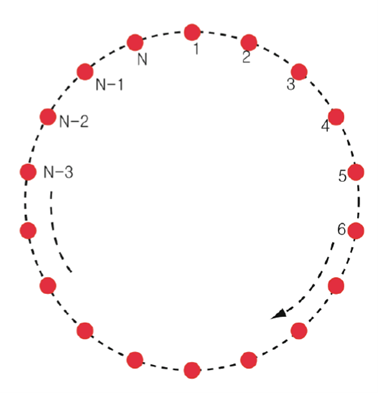
\includegraphics[width=.5\textwidth]{BKBC.png}
    \bicaption{波恩-卡门边界条件}{Born-Karman Boundary Condition}\label{BKBC}
\end{figure}

对于该模型,由于其周期性,显然有以下等式成立:
\begin{align}
    u_{N+1} &= u_1 \notag\\
    u_{N+n} &= u_n \text{。}
\end{align}

将该式带入运动方程,可以得到关于$k$的一系列取值:
\begin{equation}
    k = \frac{2\pi}{Na}m \text{,} \label{K}
\end{equation}
其中,m可以取所有整数。

由此可知,$k$的取值并不是连续的,而是一个个分立的值。%
但是由于在晶体中,$N$是一个及其大的数,因此,相较于布里渊区的大小,$k$可以当作是准连续的一个量。%
此处得到的$k$的取值,将在后面分析格波数量时起到关键作用。

\subsection{色散关系 (Dispersion Relation)} \label{DR}

将等式\ref{DRE}和\ref{K}结合起来,得到完整的色散关系表达式:
\begin{equation}
    \omega = 2 \sqrt{\frac{\beta}{m}} \left | sin \frac{ka}{2} \right | \mathrm{,} \ k = \frac{2\pi}{Na}m \text{,}\label{DREK}
\end{equation}
其中,m可以取所有整数。

色散关系反映的是波速和波长的关系,式中$\omega$和$k$分别可以作为反映波速和波长的物理量,%
因此该$\omega$ \~{} $k$关系也称为色散关系。

根据色散关系表达式,可以作出$\omega$ \~{} $k$在第一布里渊区的关系图:
\begin{figure}[htb]
    \centering
    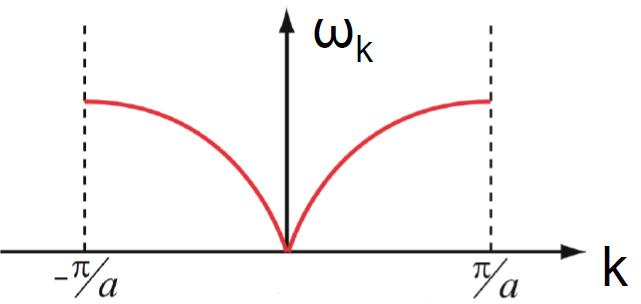
\includegraphics[width=.5\textwidth]{OmegaK.png}
    \bicaption{$\omega$ \~{} $k$在第一布里渊区的关系图}{$\omega$ \~{} $k$ in 1st B.Z.}\label{OmegaK}
\end{figure}

由简谐振荡的相关概念可知,一维单原子链中的一个原子的固有频率由下式决定:
\begin{equation}
    \omega_0 = \sqrt{\frac{\beta}{m}} \text{;}
\end{equation}
而由色散关系的表达式\ref{DREK}可知,%
一维单原子链的出现,上述谐振子的固有频率$\omega_0$被展宽为一个宽度为$2\omega_0$的频带,在这个频带中,%
可以给出频率的最大值和最小值如下:
\begin{align}
    \omega_M &= \sqrt{\frac{\beta}{m}}\\
    \omega_m &= 0 \text{。}
\end{align}

因此,可以说色散关系反映的是一维单原子链中所有原子的运动情况,它应该表征的是一些可以描述所有原子运动的物理量。%
事实上,这$N$个原子的集体行为,可以反映出一种波动(行波),这一波动称为格波,将在下一节进行讨论。

\subsection{格波 (Lattice Waves)} \label{LW}

在经典物理中,机械波可以由波矢、频率等物理量来描述,对于晶体中的格波仍然可以如此分析。%
由上一节给出的色散关系,一个确定的$k$,可以对应一个$\omega_0$,同时也就对应了晶体中的一个格波,或者是一种振动模式。

为了更加清晰地了解格波的性质,现在引入独立格波这个概念。由于晶体的周期性,可以给出:
\begin{equation}
    \omega(k) = \omega(k+G),\ G=m \cdot \frac{2\pi}{a}\hat{a} \text{,}
\end{equation}
$G$是晶体中倒空间的倒格矢,m可以取所有整数。

于是可以得知对应于$k$和$k+G$的格波,实际上具有相同的$\omega$,%
反映在原子振动上,这两条格波描述的是同一种振动模式。因此在分析过程中,可以只分析其中一条。%
将这两条格波对应同一种振动模式的格波视为一种格波,称为独立格波,此时一个$k$可以唯一对应一个格波。

将上述分析推广至整个晶体,只需要分析第一布里渊区内的格波的性质,便可以得出有关晶格振动的相关规律。%
于是我们可以把限定在第一布里渊区内的格波视为独立格波,而这些格波可以由简约波矢(位于第一布里渊区内的波矢)描述。

下面就来讨论以下在一维单原子链中,独立格波的数量问题。由波恩-卡门边界条件给出的$k$的取值表达式\ref{K},%
若限定$k$在第一布里渊区内取值,可以得出m的取值范围:
\begin{equation}
    -\frac{N}{2} \le m < \frac{N}{2} \text{,}
\end{equation}
因此m的取值个数为$N$个,在第一布里渊区内$k$的取值也只能有$N$个。
根据色散关系和独立格波的概念,在一维单原子链中,晶体中也只能有$N$个独立的振动模式或$N$个独立格波。

同时,在一维单原子链中,每个原子有一个自由度数,$N$个原子则有$N$个自由度数,于是可以得出以下等式:
\begin{equation}
    \text{总自由度数}=\text{独立格波数} \text{。} \label{3PN}
\end{equation}
可以证明,这一结论对于一维双原子链以及三维情况都是成立的,对于后面的学习十分重要。

\section{一维双原子链 (1D Diatomic Chain)}

如图 \ref{1DDC} 所示,假设一个晶格常数为a,有$N$个原胞的一维双原子链,每个原胞内有两个原子。
为研究方便,同样作一维单原子链中的假设,即简谐假设和最近邻假设。
\begin{figure}[htb]
    \centering
    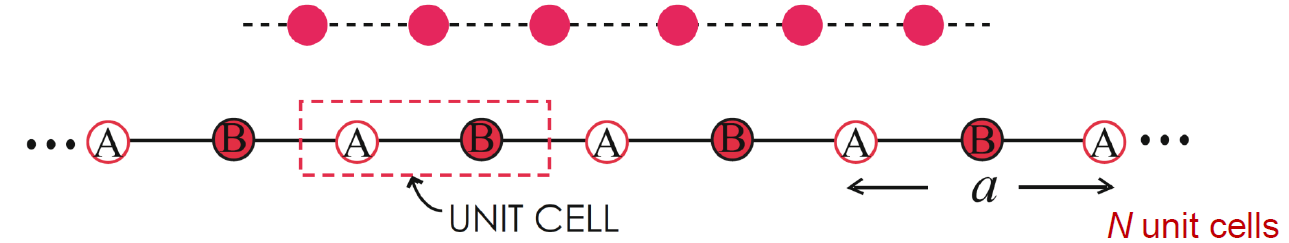
\includegraphics[width=.7\textwidth]{1DDC.png}
    \bicaption{一维双原子链}{1D Diatomic Chain}\label{1DDC}
\end{figure}

在以上假设的基础上,对该模型进行如下分析。

\subsection{运动方程 (Equation of Motion)}

类似一维单原子链,对一维双原子链中第n个原胞进行受力分析,即可得到它的运动方程。%
根据牛顿第二定律和胡克定律,有
\begin{align}
    M \ddot{u}_n &= \beta (v_n + v_{n-1} - 2u_n)\\
    m \ddot{v}_n &= \beta (u_n + u_{n+1} - 2v_n) \text{,}
\end{align}
式中$\beta$,可以由两个原子之间的作用势进行的泰勒展开后得到,这里不做讨论。%
$u_n$表示第n个原胞中一个原子的位移,$M$为该原子质量;$v_n$表示第n个原胞中另一个原子的位移,$m$为该原子质量。%
为了分析方便,假设$M>m$。如下图\ref{1DDCEOF}所示。
\begin{figure}[htb]
    \centering
    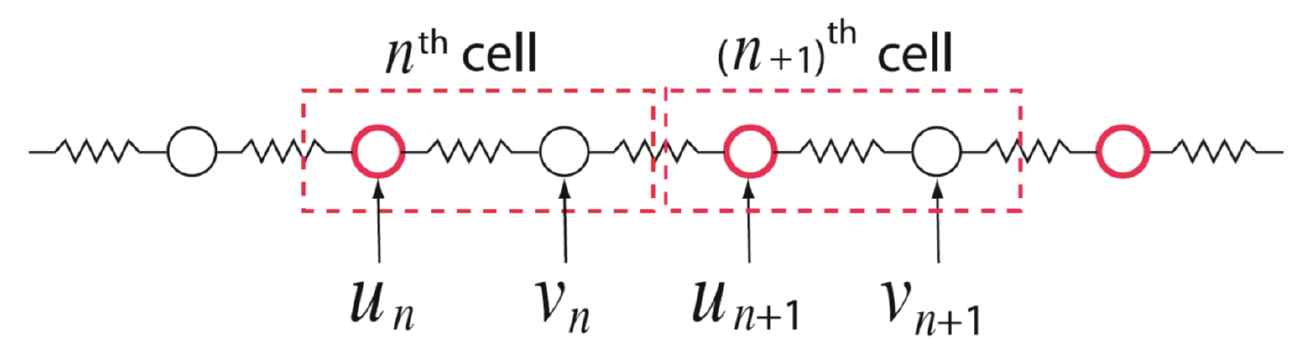
\includegraphics[width=.7\textwidth]{1DDCEOF.png}
    \bicaption{一维双原子链中的一个原胞}{A Primitive Cell in 1D Diatomic Chain}\label{1DDCEOF}
\end{figure}

下面求解这个运动方程(组)。根据二阶微分方程解的特征,可知$u_n$和$v_n$应满足:
\begin{align}
    u_n &= A e^{i(nak - \omega t)}\\
    v_n &= B e^{i[(n + \frac{1}{2}) ak - \omega t]} \text{,} \label{1DDCEOM}
\end{align}
将其带回原方程,可得一个线性齐次代数方程组:
\begin{equation}
    \begin{cases}
        (2 \beta - M \omega ^2)A-2 \beta \cos (\frac{1}{2}ak)B = 0,\\
        -2\beta\cos (\frac{1}{2}ak)A + (2\beta - m \omega ^2)B = 0 \text{。}
    \end{cases}
\end{equation}

要使该代数方程组有$A$和$B$的非零解,从而使得运动方程的表达式有意义,%
需要将$A$和$B$当作求解变量,列出其系数行列式并令该行列式的值为零,于是有:
\begin{equation}
    \begin{vmatrix}
        2 \beta - M \omega ^2 & -2 \beta \cos (\frac{1}{2}ak)\\
        -2\beta\cos (\frac{1}{2}ak) & 2\beta - m \omega ^2
    \end{vmatrix}
    =0 \text{。}
\end{equation}

由上式可得$\omega^2$ \~{} $k$关系,亦即色散关系:
\begin{equation}
    \omega^2_\pm=\frac{\beta}{Mm}[(M+m)\pm\sqrt{M^2+m^2+2Mm\cos(ak)}] \text{。} \label{1DDCDR}
\end{equation}

式中,取$+$时,表示$\omega_+^2$,此时对应较高的频率;取$-$时,表示$\omega_-^2$,此时对应较低的频率。

与一维单原子链中相同,一维双原子链依据波恩-卡门边界条件也可以得到关于$k$的一系列取值:
\begin{equation}
    k = \frac{2\pi}{Na}m \text{,} \label{1DDCK}
\end{equation}
其中,m可以取所有整数。

\subsection{色散关系 (Dispersion Relation)}

将式\ref{1DDCDR}中的$\omega_+^2$和$\omega_-^2$分开写,再次叙述这一色散关系:
\begin{align}
    \omega^2_+&=\frac{\beta}{Mm}[(M+m)+\sqrt{M^2+m^2+2Mm\cos(ak)}]\\
    \omega^2_-&=\frac{\beta}{Mm}[(M+m)-\sqrt{M^2+m^2+2Mm\cos(ak)}] \text{。}
\end{align}

根据色散关系表达式,可以作出$\omega$ \~{} $k$的关系图:
\begin{figure}[htb]
    \centering
    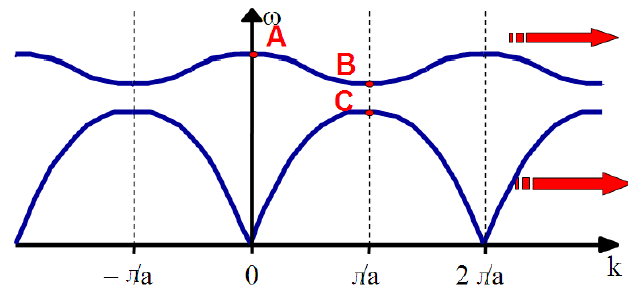
\includegraphics[width=.4\textwidth]{1DDCDR.png}
    \bicaption{$\omega$ \~{} $k$的关系图}{$\omega$ \~{} $k$}
\end{figure}

图中,位于上方的曲线就是高频的$\omega_+$,位于下方的曲线就是低频的$\omega_-$。%
这与一维单原子链中的情况略有不同,此时在图中存在两条$\omega$ \~{} $k$的曲线。

下面,类似一维单原子链中的处理方法,我们只在第一布里渊区中讨论独立格波的一些性质。
\begin{figure}[htb]
    \centering
    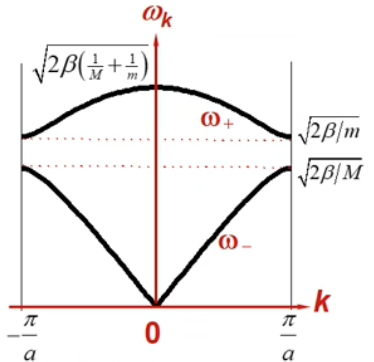
\includegraphics[width=.33\textwidth]{1DDCDR1.png}
    \bicaption{$\omega$ \~{} $k$在第一布里渊区的关系图}{$\omega$ \~{} $k$ in 1st B.Z.} \label{1DDCDR1}
\end{figure}

如图\ref{1DDCDR1}所示,其描述了在第一布里渊区内的$\omega$随$k$的变化趋势。%
其中,在$k=0$和$k=\pm\frac{\pi}{a}$处,$\omega$取到极大值或极小值,如下表所示:
\begin{table}[htb]
    \centering
    \bicaption{$\omega$的极大值或极小值}{The Maximum or Minimum of $\omega$}\label{DRT}
    \begin{tabular}{|c|c|c|}
        \hline
                             & $\omega_+$                               & $\omega_-$                \\ 
        \hline
        $k=0$                & $\sqrt{2\beta(\frac{1}{M}+\frac{1}{m})}$ & $0$                       \\ 
        \hline
        $k=\pm\frac{\pi}{a}$ & $\sqrt{\frac{2\beta}{m}}$                & $\sqrt{\frac{2\beta}{M}}$ \\ 
        \hline
    \end{tabular}
\end{table}

讨论完其数学特征,下面来看一下这一曲线有何具体的物理含义。%
在晶格动力学中,上面提到的高频的$\omega_+$称为光学支(Optical Branch),低频的$\omega_-$称为声学支(Acoustical Branch)。%
光学支和声学支中间的部分称为所谓的“禁带”,在该频率区间不存在振动。

这两种不同频率的分支,也可以反映到原胞中原子的具体振动情况。%
对于光学支,反映的是在一个原胞中两个原子振动方向相反;对于声学支,反映的是在一个原胞中两个原子振动方向相同。%
上述结论可以直接由$\frac{u_n}{v_n}$的正负性得到,具体的计算过程就不再这里赘述了。

当原胞中两个原子振动方向相反时,如果光学支的平均振动频率与外界电磁波的频率相当,那么晶体可能会发生共振吸收,从而对晶体的光学性质产生影响,%
因此称之为光学支;当原胞中两个原子振动方向相同时,原胞内的原子的相对运动较弱,而原胞的整体运动恰与声波在晶体中传播的特点相吻合,%
因此称之为声学支。

当然,以上只不过是非常简单的定性分析,对原子振动状态的定量分析和极值点处的特殊振动状态的分析在本节从略。%
下面再大致了解一下一维双原子链中格波的特点。

\subsection{格波 (Lattice Waves)}

一维双原子链中格波特点的分析过程和一维单原子链的分析过程完全一致,下面通过一张表格给出一维双原子链中的一些数量关系:
\begin{table}[htb]
    \centering
    \bicaption{一维双原子链中的数量关系}{Quantity Relations in 1D Diatomic Chain}
    \begin{tabular}{|c|c|}
        \hline
        \multicolumn{2}{|c|}{一维双原子链}  \\ 
        \hline
        原胞数        & $N$                 \\ 
        \hline
        晶格振动波矢数 & $N$                 \\ 
        \hline
        原胞内原子数   & $2$                 \\ 
        \hline
        总自由度数     & $2N$                \\ 
        \hline
        独立格波数     & $2N$                \\ 
        \hline
        分支          & $2$                 \\ 
        \hline
        分支情况      & 一支声学波,一支光学波\\ 
        \hline
    \end{tabular}
\end{table}

可以看到,在一维双原子链中,原胞数和第一布里渊区的波矢数相等,这在之前已经证明过;%
在一维条件下,每个原子有一个自由度数,此处总共$2N$个原子,因此总自由度数为$2N$,其恰好等于独立格波数,%
这与式\ref{3PN}相符。

此外,注意到此处格波的分支数为2,分为一支光学波和一支声学波,可以猜测有
\begin{equation}
    \text{分支数} = \text{原胞内原子数} \times \text{维数,} \label{Bran}
\end{equation}
成立,这一关系对于后续分析三维晶体也有帮助。

\newpage

\section{三维晶体 (3D Crystal)}

常见的三维晶体如铁、铜等金属,可以归为三维单原子链(三维单原子晶体),%
如钙钛矿、金刚石、闪锌矿等,可以归为三维P原子链(三维晶体),对于前面三种晶体,P依次等于5、2、2。

通过前面两节对一维单原子链和一维双原子链的分析,作适当的推广,可以得到如下表格中的结论:
\begin{table}[htb]
    \centering
    \bicaption{三维晶体中的数量关系}{Quantity Relations in 3D Crystal}
    \begin{tabular}{|c|c|c|c|c|c|c|c|}
        \hline
         & 原胞数 & \makecell[c]{晶格振动\\[-7pt]波矢数} & \makecell[c]{原胞内\\[-7pt]原子数} & \makecell[c]{总自由\\[-7pt]度数} & \makecell[c]{独立\\[-7pt]格波数} & 分支数 & 分支情况 \\ 
        \hline
        \makecell[c]{一维单\\[-7pt]原子链} & $N$   & $N$           & 1           & $N$       & $N$       & 1      & 1支声学波 \\ 
        \hline
        \makecell[c]{一维双\\[-7pt]原子链} & $N$   & $N$           & 2           & 2$N$      & 2$N$      & 2      & \makecell[c]{1支声学波\\[-7pt]1支光学波} \\ 
        \hline
        \makecell[c]{一维P\\[-7pt]原子链}  & $N$   & $N$           & P           & P$N$      & P$N$      & P      & \makecell[c]{1支声学波\\[-7pt]P-1支光学波} \\ 
        \hline
        \makecell[c]{三维单\\[-7pt]原子链} & $N$   & $N$           & 1           & 3$N$      & 3$N$      & 3      & \makecell[c]{3支声学波\\[-7pt](1纵2横)} \\  
        \hline
        \makecell[c]{三维P\\[-7pt]原子链}  & $N$   & $N$           & P           & 3P$N$     & 3P$N$     & 3P     & \makecell[c]{3支声学波\\[-7pt](1纵2横)\\[-7pt]3P-3支光学波} \\ 
        \hline
    \end{tabular}
\end{table}

值得注意的是,在三维晶体中,每个原子有三个自由度数,此处总共P$N$个原子,因此总自由度数为3P$N$,其恰好也等于独立格波数,%
因此总自由度数和独立格波数的相等关系对于三维晶体是成立的。

而式\ref{Bran}所描述的分支数的关系,显然对于三维晶体也是成立的。

以金刚石结构的Si晶体为例,它是一个三维的、每个原胞内有2个原子的晶体,%
假设其含有$N$个原胞,独立格波数为$3 \times 2  \times N= 6N$个,则分支数为$3 \times 2 = 6$支。%
这6支格波中,有3支是声学波,3支是光学波,分别都是1纵2横(1个纵波,2个横波),如图\ref{Si}所示。
\begin{figure}[htb]
    \centering
    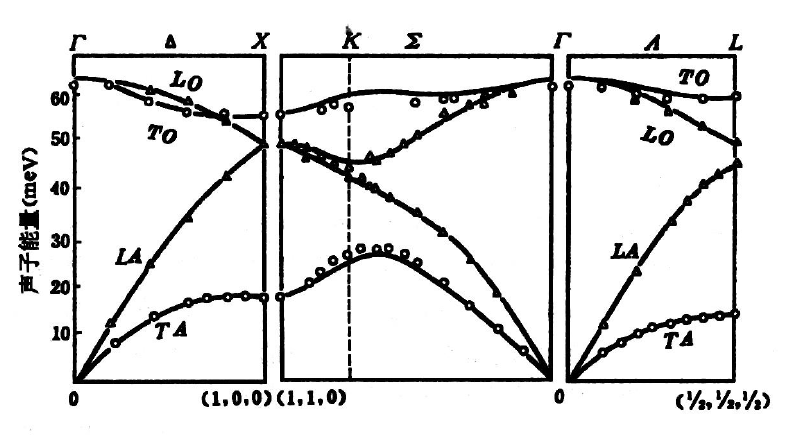
\includegraphics[width=.7\textwidth]{Si.png}
    \bicaption{Si晶体中的色散关系}{$ω_\mathbf{k}$ of Si Crystal} \label{Si}
\end{figure}

因为在Si晶体中,声学波和光学波中的两支横波的色散关系是重叠的,因此在图中只能看到四条曲线。

值得注意的是,在图\ref{Si}中,纵坐标表示的物理量是声子能量,而不是格波的振动频率$ω$。%
事实上,在温度一定的条件下,声子能量和格波的振动频率$ω$有着一一对应的关系。%
下面就来介绍声子的概念。

\section{格波的量子化 (Quantization of Lattice Waves)}

这一节的任务就是完成格波的量子化过程,具体而言是将格波的能量进行量子化。%
在这一过程中,将会引入声子的概念,这对于研究晶体的热学性质,以及和晶体中原子运动相关的其他性质都是非常重要的。

\subsection{振动模式和谐振子的等价性 (Equivalence Between A Vibration Mode and A Harmonic Oscillator)}

通过以上对格波概念理解的深入,会产生一个很自然的想法就是格波的能量,也就是晶格振动的能量到底该如何求解。%
因为如果想要得到晶体的热容,必然需要得到一个能量和温度的关系式。

下面还是以一维单原子链为例,尝试去分析晶格振动的总能量。%

在一维单原子链中,对于一个特定的振动模式,也就是对应某一个波矢$k$,其能量满足以下关系式:
\begin{equation}
    E_k=T_k+U_k=\frac{1}{2}m\sum\dot{u}_n^2+\frac{1}{2}\beta\sum(u_{n-1}-u_n)^2 \text{。}
\end{equation}

将式\ref{EOM}带入上式,可以得到动能的表达式:
\begin{equation}
    T_k=-\frac{1}{2}m\omega^2e^{-2i\omega t}\sum_{n=1}^{N}e^{2ikna} \text{。}
\end{equation}

而由势能和作用力的关系,以及色散关系,又可以得到势能的表达式:
\begin{equation}
    U_k=\frac{1}{2}m\omega^2e^{-2i\omega t}\sum_{n=1}^{N}e^{2ikna} \text{。}
\end{equation}

要完成上述计算,并求得对应所有波矢的振动模式能量的加和,从而得到晶格振动的总能量是十分困难的。%
因此,需结合分析力学的相关知识,引入广义坐标$q_k$和广义动量$p_k$:
\begin{align}
    q_k &= \sqrt{m}\sum_{n=1}^{N}e^{-i(\omega t-kna)} \\
    p_k &= \frac{\mathrm{d}q_k}{\mathrm{d}t} = -i\omega \sqrt{m}\sum_{n=1}^{N}e^{-i(\omega t-kna)} \text{,} 
\end{align}
将其带入动能和势能的表达式,有:
\begin{align}
    T_k &= \frac{1}{2}p_k^2 \\
    U_k &= \frac{1}{2}\omega^2q_k^2 \text{。} 
\end{align}

因此,动能的表达式最终化为:
\begin{equation}
    E_k=T_k+U_k=\frac{1}{2}p_k^2 + \frac{1}{2}\omega^2q_k^2 \text{。} 
\end{equation}

而这一形式,恰恰符合一个具有位置$q_k$、动量$p_k$和频率$\omega$的谐振子的能量的表达式。

这一事实告诉我们,对于一个有$N$个原子的一维单原子链,它的晶格振动的总能量可以表达成$N$个谐振子能量的加和。%
将其推广至三维晶体,可以得到,对于一个有$N$个原子的三维晶体,它的晶格振动的总能量可以表达成3$N$个谐振子能量的加和,%
而这3$N$个谐振子的频率与3$N$个独立格波的频率相等。

概括而言,一个独立格波,也就是一个独立振动模式,从能量而言,对应了一个频率与之相等的谐振子。

\subsection{声子 (Phonon)}

接下来的问题自然就变成了要如何获得上述谐振子的能量。在固体物理课上,给出过谐振子的能量表达式,这里直接引用该结论:
\begin{equation}
    E_n=(n + \frac{1}{2})\hbar \omega \text{,} \label{HO}
\end{equation}
其中,$n$可以取所有非负整数。

由此可知,谐振子的能量是被量子化的,它的最低的能量为当$n=0$时的$\frac{1}{2} \hbar \omega$。

既然谐振子的能量满足上述表达式,那么晶格振动的能量是否也会有相类似的形式?%
下面就引入声子这个概念,从量子化的角度重新认识晶格振动的能量。

类似式\ref{HO},对于一个振动频率为$\omega_j(k)$的格波或振动模式,其具有的能量为:
\begin{equation}
    E_j(\mathbf{k}) = (n_j(\mathbf{k}) + \frac{1}{2})\hbar \omega_j(\mathbf{k}) \text{,} \label{EOL}
\end{equation}
其中,$n_j(\mathbf{k})$可以取所有非负整数。%
$\mathbf{k}$表示波矢,$k$表示波矢的大小,下标$_j$表示对应于某个k的格波的不同分支。

因此,对式\ref{EOL}求加和,便可以得到对于一个具有$N$个原胞,每个原胞含有P个原子的晶体的晶格振动总能量:
\begin{equation}
    E = \sum_{j=1}^{3P}\sum_{k=1}^{N}E_j(\mathbf{k}) = \sum_{j=1}^{3P}\sum_{k=1}^{N}(n_j(\mathbf{k}) + \frac{1}{2})\hbar \omega_j(\mathbf{k}) \text{。} \label{EOC}
\end{equation}

由此,定义晶格振动的能量子
\begin{equation}
    \hbar \omega_j(\mathbf{k})
\end{equation}
为声子。

声子有特点如下:
\begin{enumerate}
    \item 声子是只能在晶体中存在的准粒子,并不是真实存在的粒子,因为准粒子描述的整个系统的性质,而不是描述系统的单个粒子的行为。
    \item 声子具有准动量$\hbar \mathbf{k}$,并不是真实的动量。
    \item 声子是一种玻色子,其数量是可变的,为$n_j(\mathbf{k})$,遵循玻色-爱因斯坦分布(B-E Distribution)。
\end{enumerate}

在研究光子、电子与格波的相互作用的时候,可以描述为它们与声子的相互作用,这对于晶体中微观粒子运动的分析有重要意义。

\subsection{晶体振动能量 (Lattice Vibration Energy)}

显然,由式\ref{EOL},研究晶体振动能量能量的问题,最终就转换为讨论$n_j(\mathbf{k})$取值的问题。

结合统计物理的相关知识

% 正文后部分
\backmatter
% 导入参考文献 (需要通过 latexmk 编译后才能显示)
\PrintReference

\end{document}